% --------------------------------------|
% -------------------------------------|
% ------------------------------------|
\section{Investigación} 
% ------------------------------------\
% --------------------------------------\
% ----------------------------------------\


% --------------------------------------|
% -------------------------------------|
\subsection{BFS}
\begin{center}
    ¿Cuál es la diferencia entre Backtracking y el algoritmo de búsqueda BFS?
\end{center}
% --------------------------------------\
% ----------------------------------------\



\noindent \textbf{\large{Explicación del algoritmos BFS (Breadth First Search):}}\\ 


Es un algoritmo de búsqueda no informada utilizado que se utiliza para buscar o recorrer
en grafos principalmente generalmente sobre árboles. Comienza en la raíz del árbol 
y visita todos los nodos en el nivel de profundidad actual antes de pasar a los 
nodos en el siguiente nivel de profundidad. El único inconveniente aquí es que,
cuando son grafos completos estos pueden contener ciclos, por lo que podemos estar en 
círculos. Para evitar procesar un nodo más de una vez, dividimos los vértices en 
dos categorías: visitado y no visitado. Utilizando una matriz para marcar los vértices 
visitados y suponemos que todos los nodos estan unidos. BFS utiliza una estructura
de datos en cola para el recorrido.

\subsubsection*{Como funciona }

\begin{enumerate}
    \item \textbf{Inicialización}: Comienza desde el vértice fuente $s$.
    \item \textbf{Exploración sistemática}: Explora los vértices de $G$ para descubrir todos los vértices alcanzables desde $s$, expandiendo uniformemente la frontera entre lo descubierto y lo no descubierto.
    \item \textbf{Cálculo de distancias}: Calcula la distancia (menor número de vértices) desde $s$ a todos los vértices alcanzables. Esto se hace durante la exploración, manteniendo un registro de las distancias mientras se avanza en el grafo.
    \item \textbf{Construcción del árbol}: Produce un árbol con raíz en $s$ que contiene a todos los vértices alcanzables. Este árbol BF representa la estructura de exploración y los caminos más cortos desde $s$.
    \item \textbf{Camino más corto}: El camino desde $s$ a cada vértice en este árbol contiene el mínimo número de vértices. Es el camino más corto medido en número de vértices.
\end{enumerate}

\subsubsection*{Pseudocódigo \cite{bfsps}}

\begin{verbatim}
    1  método BFS(Grafo,origen):
    2      creamos una cola Q
    3      agregamos origen a la cola Q
    4      marcamos origen como visitado
    5      mientras Q no este vacío:
    6          sacamos un elemento de la cola Q llamado v
    7          para cada vertice w adyacente a v en el Grafo: 
    8              si w no ah sido visitado:
    9                 marcamos como visitado w
    10                 insertamos w dentro de la cola Q
\end{verbatim}


\subsection*{Diferencias con Backtracking}


\begin{enumerate}
    \item Objetivo
    \begin{itemize}
        \item \textbf{Backtracking:} Encontrar todas las soluciones posibles
        \item \textbf{BFS:} Encontrar la ruta más corta
    \end{itemize}
    \item Estructuras de datos
    \begin{itemize}
        \item \textbf{Backtracking:} Funciona principalmente con recursión (aun que no es una ED)
        \item \textbf{BFS:} Usa una cola para realizar los recorridos
    \end{itemize}
    \item Alcance 
    \begin{itemize}
        \item \textbf{Backtracking:} Como busca en todas las soluciones posibles el retroceso lo hace al alcanzar un punto muerto
        \item \textbf{BFS:} Hace un recorrido en profundidad lo cual determina si avanza o no, así encuentra la ruta más corta
    \end{itemize}
    \item Memoria
    \begin{itemize}
        \item \textbf{Backtracking:} Menos memoria porque solo actualiza su estado de búsqueda
        \item \textbf{BFS:} Más memoria porque en grafos muy grandes, la cola créese demasiado 
    \end{itemize} 
    \item Donde usar
    \begin{itemize}
        \item \textbf{Backtracking:} Problemas de búsqueda como las N reinas
        \item \textbf{BFS:} Problemas de búsqueda de ruta más corta
    \end{itemize}    
\end{enumerate}


% --------------------------------------|
% -------------------------------------|
\subsection{DFS}
\begin{center}
    ¿Cuál es la diferencia entre Backtracking y el algoritmo de búsqueda DFS?
\end{center}
% --------------------------------------\
% ----------------------------------------\

\noindent \textbf{\large{Primero expliquemos que es el algoritmos DFS (Depth First Search):}}

Es un algoritmo utilizado en la teoría de grafos para buscar y recorrer grafos o árboles, 
no utiliza información sobre el costo de los movimientos o la ubicación de la meta.\\


El recorrido comienza revisando el nodo actual (la raíz si es un árbol o seleccionando un 
nodo arbitrario si no), después se mueve a uno de sus sucesores para repetir el proceso y 
explora tanto como sea posible en esa rama, si el nodo actual no tiene sucesor a revisar, 
regresamos a su predecesor y el proceso continua, es decir se mueve a otro sucesor del nodo, 
si la meta o solución es encontrada la búsqueda termina.

\begin{itemize}
    \item Pseudocódigo: El algoritmo DFS puede tener una implementación recursiva o iterativa 
    (utilizando pilas), a continuación esta el pseudocodigo de la implementación recursiva:
    \begin{center}
        \begin{algorithmic}[1]
            \Procedure{DFS}{$\text{vertex } v$}
            \State $\text{visit}(v)$
            \ForAll{$\text{neighbor } u \text{ of } v$}
                \If{$u \text{ is undiscovered}$}
                    \State $\text{call DFS}(u)$
                \EndIf
            \EndFor
            \EndProcedure
        \end{algorithmic}
    \end{center}

    \item Gráfica: La siguiente gráfica muestra como se van descubriendo los nodos con el algoritmo DFS.

    \begin{center}
        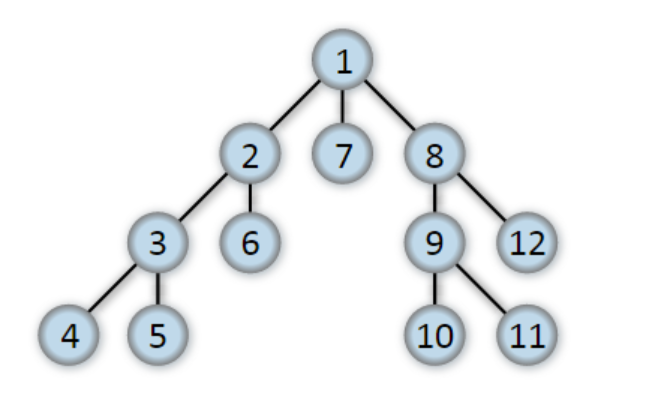
\includegraphics[scale = 0.5]{IMA/ejemploDFS.png}
    \end{center}

    \item Aplicaciones: Los principales usos que le dan al algoritmo son:
    \begin{itemize}
        \item Determinación de Conectividad: DFS se puede utilizar para determinar si un grafo es 
        conexo, es decir, si hay un camino entre cada par de nodos.

        \item Detección de Ciclos: DFS puede detectar ciclos en un grafo no dirigido. Si mientras 
        se ejecuta el algoritmo encuentra un nodo ya visitado, entonces hay un ciclo.

        \item Topological Sorting: DFS se puede utilizar para realizar una ordenación topológica 
        en un grafo dirigido, que es una lista lineal de todos los nodos tal que para cada arista 
        dirigida $uv$ de un nodo $u$ a un nodo $v$, $u$ aparece antes que $v$ en la lista.

        \item Encontrar Componentes Conectados: DFS se puede utilizar para encontrar los componentes 
        conectados de un grafo no dirigido.

        \item Resolver acertijos con una sola solución, como laberintos.
    \end{itemize}

\end{itemize}


Tiene una complejidad de O(n) en el peor de los casos y funciona mejor en árboles poco profundos.\\

\textbf{\large{Diferencias entre DFS y Backtracking}} \\

Ahora teniendo todo esto en cuenta la principal diferencia que tiene el \textbf{algoritmo DFS} 
con \textbf{backtracking} es que DFS encuentra una solución a un problema (ya que al encontrar una 
meta se deja de recorrer la gráfica) y backtracking encuentra todas las posibles soluciones de ese 
problema, entonces podemos decir que tienen diferencia en el espacio de búsqueda:\\

\begin{itemize}
    \item DFS: Se adentra tanto como sea posible en la estructura del grafo antes de retroceder 
    para explorar otras ramas.

    \item Backtracking: Explora todas las posibles soluciones de manera incremental, retrocediendo 
    cuando se alcanza una solución inválida o se agotan todas las opciones.
\end{itemize}

Es decir el backtracking evalúa exhaustivamente cada posibilidad y retrocede cuando encuentra una solución inválida, mientras que DFS se adentra en la exploración del espacio de búsqueda, pero no garantiza encontrar todas las soluciones.

% --------------------------------------\
% ----------------------------------------\